\chapter{Experimental Setup}
\label{ExperimentalSetup}
% \begin{itemize}
%     \item We aim to answer the following questions:
%     \begin{itemize}
%         \item RQ1: How do different input types (source, unstripped decompiled, demi-stripped, stripped) affect the model's performance (data-richness effect)?
%         \item RQ2: What is the impact of data duplication on the model's performance (data-duplication effect)?
%         \item RQ3: To what extent each aspect of stripped decompiled binaries impacts the model's performance (data-input study)?
%         \item RQ4: How do different pre-training objectives affect the model's performance (model-objective effect)?
%     \end{itemize}
%     \item Explain what script was used for deduplication
%     \item Explain how the model was loaded in and what configurations were used
%     \item Explain which metrics we used to assess the model
%     \item Explain the manual evaluation of the stripped code
%     \item Explain the baseline of CodeT5 on normal programming languages, and our own finetuning on source-C
% \end{itemize}

% \newpage

\section{Research Questions}
We must create and assess our model to reach our goal of creating an automatic system for decompiled code summarisation. We define research questions which will be answered throughout the thesis. Firstly it is essential to assess the different datasets and set a baseline for each. We can then investigate the impact of different aspects of the data. Finally, we can apply this knowledge to design intermediate-training objectives, further improving performance.

\begin{itemize}
    \item \textbf{RQ1: How do different input types (source, unstripped decompiled, demi-stripped, stripped) affect the model's performance? (data-richness effect)}
    \begin{sloppypar}
    Firstly, we want to know the impact of the data-richness on the model performance. The different datasets have different degrees of data richness. The source code has all of its identifiers and comments in code. Unstripped decompiled code has no comments and loses many of its identifiers. The decompiler also introduces some noise. Demi-stripped data loses all of the remaining identifiers. Stripped data also has no identifiers and introduces even more decompilation noise.
    \end{sloppypar}
    \item \textbf{RQ2: What is the impact of data duplication on the model's performance? (data-duplication effect)}
    \begin{sloppypar}
    Secondly, we will evaluate how the model reacts to data duplication, whether the model performance is simply a result of the memorisation of certain examples, or if the performance is a result of a generalisable understanding of the data.
    \end{sloppypar}
    \item \textbf{RQ3: To what extent each aspect of stripped decompiled binaries impacts the model's performance? (data-input study)}
    \begin{sloppypar}
    The different datasets each contain different aspects of the original source code. Which of these aspects are most important for the model performance? 
    \end{sloppypar}
    \item \textbf{RQ4: How do different intermediate-training objectives affect the model's performance? (model-objective effect)}
    \begin{sloppypar}
    Finally, we will apply the insights provided by the previous questions to design new intermediate-training objectives, through which we aim to address the shortcomings of the base model. 
    \end{sloppypar}
\end{itemize}

\section{Dataset}
To answer the research questions, a diverse and representative dataset must be constructed. The Buildswarm dataset contains around 1.8m aligned decompiled-sourcecode pairs as well as 400k aligned stripped-sourcecode pairs. The significant difference is caused by the inherent difficulty of finding functions in stripped decompiled code. 

From this dataset, we collect any documentation located above the functions using srcML \ref{fig:srcML}. 

\begin{figure}[H]
  \centering
  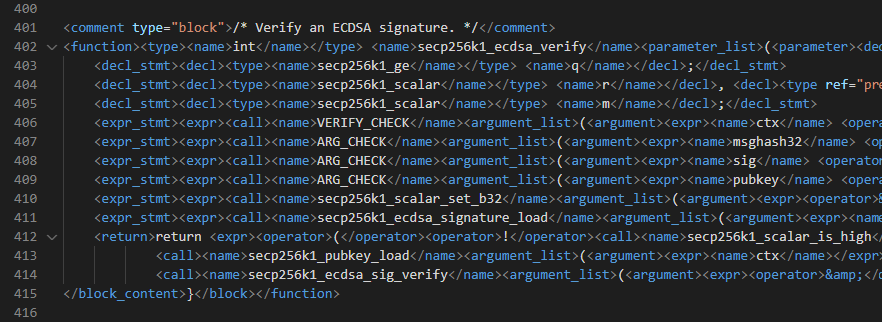
\includegraphics[width=\linewidth]{img/srcML.png}
  \caption{Example function with its documentation (truncated)}
  \label{fig:srcML}
\end{figure}

This documentation can be split into the following classes: 
\begin{enumerate}
  \item Double slash comments, example from Jep:release\_utf\_char. 
\begin{verbatim}
    // release memory allocated by jstring2char
\end{verbatim}
    These comments are thrown out, as these are generally not used for documentation.
  \item Single line comments, example from Nesbox:Curl\_mime\_read.
\begin{verbatim}
    /* Set mime part remote file name. */
\end{verbatim}
   We take the entire comment as a description.
  \item Multiline comments, example from oftc-ircservices:cs\_on\_client\_join.
\begin{verbatim}
    /**
     * CS Callback when a Client joins a Channel
     * @param args 
     * @return pass_callback(self, struct Client *, char *)
     * When a Client joins a Channel:
     *  - attach DBChannel * to struct Channel*
     */
\end{verbatim}
    In this case, we take the first line or sentence.
\end{enumerate}



The data is pre-processed using the Pandas \footnote{Pandas: \url{https://pandas.pydata.org/}} data analysis library as well as the Pandarallel \footnote{Pandarallel: \url{https://pypi.org/project/pandarallel/}} parrallelizability extention for Pandas.

The samples are pre-processed by first extracting the function name and adding it as a column to the data. For the stripped samples, the alignment with C is utilised by extracting the function name from the source code for each sample. Next, the samples are aligned with the comment data using the file name where they reside appended with the function name, for instance: \textit{/Repos\_Bionic/ secp256k1/secp256k1.c:secp256k1\_pubkey\_load}. We further pre-process the data by removing any newlines from the function body and by unescaping any characters that have been escaped for file safety purposes, such as \&gt; for $>$.

The samples are split into a train, validation and test set. Each set is collected into a single .jsonl \footnote{JSON Lines: \url{https://jsonlines.org/}} file.

\begin{figure}[H]
  \centering
\begin{lstlisting}[breaklines=true]
[
{"repo":"author/project","docstring_tokens":["Tokenized", "description"], "code_tokens":["Tokenized", "code"], "partition": "train"}
{"repo":"author/project","docstring_tokens":["Tokenized", "description"], "code_tokens":["Tokenized", "code"], "partition": "valid"}
]
\end{lstlisting}
  \caption{Example entries of a .jsonl file with two dummy entries}
  \label{fig:jsonl}
\end{figure}


To answer the second research question, the dataset must be deduplicated. The dataset is deduplicated using a fork\footnote{Near Duplicate Code Detector: \url{https://github.com/SERG-Delft/near-duplicate-code-remover}} of the near-duplicate-code-detector~\cite{allamanis_adverse}. We use this tool to compare all the functions in the dataset and to find clusters of near-duplicate functions. We randomly select one function per cluster and discard the rest from the dataset. 

% Slightly expand this 

\section{Model Configuration}
To first establish a performance baseline, we trained a CodeT5-base model on the summarisation task on source C. This can be used to compare the decompiled C, stripped decompiled C and the demi-stripped datasets to the source code. For deduplicated code, the results can be compared with the performance of CodeT5-base on the code summarisation task~\cite{CodeT5}, where the performance varies between 15.24 and 26.03 BLEU4 scores depending on the language. Based on this, we set the baseline for a usable summarisation model around a BLEU4 score of 15, with anything lower than a BLEU4 score of 10 essentially unusable. Besides the standard BLEU and EM metrics used by most code summarisation works~\cite{CodeBERT, CodeT5, CodeXGlue, PolyglotCodeBERT, CodeSumSmallLocal, recommend_summarization}, we also include METEOR and ROUGE-L. 

\begin{table}[!h]
\centering
\begin{tabular}{ll}
\hline
Package        & Version     \\ \hline
Nvidia drivers & 510.60.02   \\
cuda           & 11.6        \\
numpy          & 1.22.2      \\
tensorboard    & 2.8.0       \\
torch          & 1.9.0+cu111 \\
transformers   & 4.16.2      \\
tree-sitter    & 0.20.0      \\ 
Ghidra         & 10.0.4      \tablefootnote{It is not recommended to use Ghidra versions before 10.1 since these versions have not been patched against a Log4J RCE}\\ \hline
\end{tabular}
\caption{The most important packages and their versions}
\label{tab:packages}
\end{table}

A grid search of the optimal settings was infeasible from a time perspective, so training was performed mainly using the recommended settings. For the decompiled, stripped, and demi-stripped, the source length is doubled to 512 tokens instead of the standard 256 tokens used for the source code. This was done to compensate for the fact that the average length of decompiled and stripped functions was almost double that of the source code. We utilised two different servers for training\ref{tab:server}. The training was performed on either an NVIDIA RTX3080 with 10GB of VRAM or an NVIDIA GTX 1080ti with 11GB of VRAM. The authors of CodeT5 used an NVIDIA A100 GPU with 40G of VRAM for fine-tuning~\cite{CodeT5}. To compensate for the lack of memory, we reduced the batch size to 2, which was the maximum length that still fit both GPUs \ref{tab:modelSettings}.

\begin{table}[!h]
\centering
\begin{tabular}{l|ll}
\hline
                & CodeT5-base & Our Settings            \\ \hline
Source length   & 256 Tokens  & \textbf{256/512 Tokens} \\
Target length   & 128 Tokens  & 128 Tokens              \\
Max epochs      & 15          & 15                      \\
Patience        & 2           & 2                       \\
Batch Size      & 32          & \textbf{2}              \\
Vocabulary Size & 32100       & 32100                  
\end{tabular}
\caption{Model configuration of the base model and our used settings}
\label{tab:modelSettings}
\end{table}

\begin{table}[!h]
\centering
\begin{tabular}{l|ll}
\hline
        & Server 1           & Server 2                     \\ \hline
CPU     & Intel XEON E5-2620 & AMD Ryzen Threadripper 3990X \\
Cores   & 16 (32 threads)    & 64 (128 threads)             \\
RAM     & 192GB              & 128GB                        \\
GPU     & Nvidia GTX 1080TI  & Nvidia RTX 3080              \\
VRAM    & 11GB               & 10GB                         \\
Storage & 7.3TB HDD          & 1TB NVME SSD                
\end{tabular}
\caption{Hardware used for training and evaluation}
\label{tab:server}
\end{table}

\section{Manual Evaluation}
To investigate the third research question, the results of the different datasets are compared to see the influence of the different aspects of code on the model performance. Furthermore, we observe that there could be two principal reasons for a sample to be malformed. Firstly, Ghidra can fail to decompile the function correctly. Secondly, during the data collection phase, the comment might not have been appropriately parsed, which results in an incorrect description of the function. To investigate this influence on the stripped model's performance, we randomly sample 25 high and low-performing samples (in terms of BLEU-4 score) and manually analyse the decompiled code and the description. 

\section{Intermediate-Training}

We constructed three intermediate-training objectives to answer the fourth and final research question.

\subsection{Translation}
The first defined intermediate-training task is a Neural Machine Translation task. In this code-to-code task, the model has to translate the source code from one programming language to another~\cite{CodeXGlue}. 
We implemented a translation from demi-stripped to unstripped decompiled code in our case. Note that, by construction, the only difference between decompiled and demi-stripped code is the lack of identifiers in the demi-stripped code.

\begin{figure}[H]
  \centering
\begin{lstlisting}
repo: NLnetLabs\ldns
input: "undefined8 MASK0 ( long param_1 ) { 
    undefined8 uVar1; 
    if (param_1 != 0) { 
        uVar1 = MASK1(); 
        uVar1 = MASK2(uVar1); 
        return uVar1; 
    } 
    return 0; 
}"
target: "uint8_t ldns_rr_label_count (const ldns_rr * rr ){ 
    if (!rr) { 
        return 0;
    } 
    return ldns_dname_label_count (ldns_rr_owner(rr));
}"
\end{lstlisting}
  \caption{Translation intermediate training objective}
  \label{fig:tanslation}
\end{figure}

\subsection{Deobfuscation}
The second defined task is a deobfuscation objective. In this code-to-text objective, the model is tasked with predicting the identifiers in demi-stripped code. Recall that in the demi-stripped code, all identifiers are masked with meaningless placeholders, where duplicate identifiers are assigned the same placeholder. The model will have to output a map of the placeholders to their original value. While the output of the model is somewhat textual and not code, it is not precisely natural language.

\begin{figure}[H]
  \centering
\begin{lstlisting}
repo: NLnetLabs\ldns
input: "undefined8 MASK0 ( long param_1 ) { 
    undefined8 uVar1; 
    if (param_1 != 0) { 
        uVar1 = MASK1(); 
        uVar1 = MASK2(uVar1); 
        return uVar1; 
    } 
    return 0; 
}"
target: "{MASK0: ldns_rr_label_count, MASK1:
ldns_rr_owner, MASK2: ldns_dname_label_count}"
\end{lstlisting}
  \caption{Deofbuscation intermediate training objective}
  \label{fig:dobf}
\end{figure}


\subsection{Span Prediction}
Finally, we define a Span Prediction objective. The model is tasked with recovering the identifiers from demi-stripped code in this code-to-text objective. Although, unlike the DOBF objective, every identifier (even matching identifiers) is assigned unique placeholders, the model has to output the assignment of the placeholders in a form closer to natural language and puts more emphasis on duplicated identifiers which might be more critical.


\begin{figure}[H]
  \centering
\begin{lstlisting}
repo: NLnetLabs\ldns
input: "undefined8 MASK0 ( long param_1 ) { 
    undefined8 uVar1; 
    if (param_1 != 0) { 
        uVar1 = MASK1(); 
        uVar1 = MASK2(uVar1); 
        return uVar1; 
    } 
    return 0; 
}"
target: "MASK0 ldns_rr_label_count MASK1
ldns_rr_owner MASK2 ldns_dname_label_count"
\end{lstlisting}
  \caption{Span-detection intermediate training objective}
  \label{fig:spanDetection}
\end{figure}

